\documentclass[a4paper,10pt]{article}
\usepackage[utf8]{inputenc}
\usepackage[spanish]{babel}
\usepackage[affil-it]{authblk}
\usepackage{enumerate}
\usepackage{graphicx}
\usepackage{hyperref}
\usepackage{amsmath}
\usepackage{amssymb}
\usepackage{cancel}
\usepackage[usenames, dvipsnames]{color}
\usepackage{tikz}
\usepackage[labelfont=bf]{caption}
\usepackage{subcaption} %Multiple images
\usepackage{multicol} % Multiple columns
\usepackage{float}
\usepackage{cleveref}
 \usepackage{relsize} % bigger math symbols
\usepackage[margin=1.4in]{geometry}
\usepackage[titletoc,toc,title]{appendix}
\usepackage{enumitem}
\usepackage{etoolbox}
\usepackage{mdframed} %frame theorems
\usetikzlibrary{calc}
\numberwithin{equation}{section}

% Enviroment for theorems
\newmdtheoremenv[frametitle=Teorema]{theo}{Theorem}

% Circled words
\newcommand{\circled}[2][]{%
  \tikz[baseline=(char.base)]{%
    \node[shape = circle, draw, inner sep = 1pt]
    (char) {\phantom{\ifblank{#1}{#2}{#1}}};%
    \node at (char.center) {\makebox[0pt][c]{#2}};}}
\robustify{\circled}

%Appendices in spanish
\renewcommand{\appendixname}{Ap\'endices}
\renewcommand{\appendixtocname}{Ap\'endices}
\renewcommand{\appendixpagename}{Ap\'endices}

%Zero delimiter
\newcommand{\zerodel}{.\kern-\nulldelimiterspace}

%Columns separation
\setlength{\columnsep}{1cm}

%Indentation
\setlength{\parindent}{0ex}

%Multiple References

\crefrangelabelformat{equation}{(#3#1#4--#5\crefstripprefix{#1}{#2}#6)}

\usepackage{xparse}

%Boxes

\newcommand*{\boxcolor}{blue}
\makeatletter
\renewcommand{\boxed}[1]{\textcolor{\boxcolor}{%
\tikz[baseline={([yshift=-1ex]current bounding box.center)}] \node [rectangle, minimum width=1ex,rounded corners,draw] {\normalcolor\m@th$\displaystyle#1$};}}
 \makeatother

%Constantes
\newcommand{\euler}{\mathrm{e}}
\newcommand{\im}{i}

%Lemas, teoremas, definiciones y pruebas
\newcommand{\definicion}{\textbf{Definición: }}
\newcommand{\lema}{\textbf{Lema: }}
\newcommand{\teorema}{\textbf{Teorema: }}
\newcommand{\prueba}{\textbf{Prueba: }}
\newcommand{\proposicion}{\textbf{Proposición: }}
\newcommand{\corolario}{\textbf{Corolario: }}

% Definición de las secciones y su numeración

\makeatletter
\def\@seccntformat#1{%
  \expandafter\ifx\csname c@#1\endcsname\c@section\else
  \csname the#1\endcsname\quad
  \fi}
\makeatother

%opening
\title{Examen Predoctoral de Mecánica Clásica. \\
Semestre 2016-I.}
\author{Favio Vázquez\thanks{Correo: favio.vazquezp@gmail.com}}\affil{Instituto de Ciencias Nucleares. Universidad Nacional Autónoma de México.}
\date{}

\begin{document}

\makeatletter
\def\@maketitle{%
  \newpage
  \null
  \vskip 2em%
  \begin{center}%
  \let \footnote \thanks
    {\Large\bfseries \@title \par}%
    \vskip 1.5em%
    {\normalsize
      \lineskip .5em%
      \begin{tabular}[t]{c}%
        \@author
      \end{tabular}\par}%
    \vskip 1em%
    {\normalsize \@date}%
  \end{center}%
  \par
  \vskip 1.5em}
\makeatother

\maketitle

\section{Preguntas teóricas}

\subsection{Pregunta teórica 1}

Sobre las formulaciones de la mecánica, discuta los siguientes puntos:

\begin{enumerate}[label=\alph*)]
 \item Bajo qué condiciones las ecuaciones de Euler-Lagrange determinan todas las aceleraciones del
 sistema.
 \item En el caso Hamiltoniano, cuál es la condición equivalente.
 \item Dentro del formalismo de Hamilton-Jacobi qué garantiza el que la funcional generadora
 proporcione una solución de las ecuaciones de Hamilton.
\end{enumerate}

\vspace{.3cm}

\underline{Solución:} \vspace{.3cm}

\begin{enumerate}[label=\alph*)]
 \item R:
\end{enumerate}

La formulación lagrangiana en coordenadas generalizadas es equivalente a la formulación 
newtoniana, por lo tanto la ley de la naturaleza se expresa como una ecuación diferencial 
de segundo orden. Por lo tanto, para poder determinar completamente el estado 
de un sistema mecánico, y definir unívocamente todas las aceleraciones del mismo 
requerimos conocer simultáneamente las coordenadas y las velocidades en un instante 
dado. Entonces ya que las ecuaciones de Euler-Lagrange, contienen derivadas 
sobre la lagrangiana que depende de las coordenadas, las velocidades y 
posiblemente el tiempo, al conocer simultáneamente las coordenadas y velocidades 
en un instante dado, podremos determinar todas las aceleraciones del sistema.

\begin{enumerate}[label=\alph*)]
  \setcounter{enumi}{1}
 \item R:
\end{enumerate}

En el caso de la formulación hamiltoniana, ya que es equivalente a la formulación 
lagrangiana y por lo tanto a la newtoniana, se cumplen las mismas condiciones. Ahora 
en este caso, debido a que las ecuaciones de Hamilton contemplan derivadas de la 
hamiltoniana del sistema, y ésta depende de coordenadas e impulsos, se deben conocer 
ahora en un instante dado simultáneamente las coordenadas y los impulsos del sistema 
mecánico para determinar todas las aceleraciones del mismo. Debido a la relación 
directa entre los impulsos y las velocidades en esta formulación, esta condición 
se puede considerar idéntica a la anterior, aunque es un poco más formal hablar de 
impulsos en este caso, ya que la formulación hamiltoniana existe en el ámbito del 
espacio fase de coordenadas e impulsos.

\begin{enumerate}[label=\alph*)]
  \setcounter{enumi}{3}
 \item R:
\end{enumerate}

Lo que nos garantiza, en la formulación de Hamilton-Jacobi, que la funcional generadora 
proporcione una solución de las ecuaciones de Hamilton, es que ésta sea una integral 
completa, es decir que sea una solución de la ecuación en derivadas parciales resultante 
en esta formulación, que contenga tantas constantes arbitrarias independientes como 
variables independientes existan. Y debido a que en la ecuación de Hamilton-Jacobi 
las variables independientes son las coordenadas y el tiempo, para un sistema de 
$n$ grados de libertad, una integral completa debe contener $n+1$ constantes arbitrarias. 
Estas constantes que se deben obtener en el ámbito de una integral completa, nos permitirán 
expresar a las coordenadas y los impulsos como funciones del tiempo, y las constantes, 
con lo cual se puede demostrar que estas variables cumplirán con ecuaciones 
diferenciales que tienen forma hamiltoniana.

\subsection{Pregunta Teórica 2}

Considere un cuerpo rígido con momentos de inercia $I_1 > I_2 > I_3$. Si sobre el cuerpo no se 
ejercen torcas, ¿qué ejes del cuerpo son estables e inestables bajo pequeñas perturbaciones y 
por qué?

\vspace{.3cm}

\underline{Solución:} \vspace{.3cm} 

Debemos ver en qué casos, con respecto a la dirección de la velocidad angular, el 
movimiento será estable y con respecto a qué eje principal. Partimos de las ecuaciones 
de Euler para un cuerpo rígido al cual no se le aplican torcas,

\begin{align}
 \label{eq:pregunta2eq1}
 I_1\dot{\omega}_1 - \omega_2\omega_3(I_2 - I_3) = 0, \\
 \label{eq:pregunta2eq2}
 I_2\dot{\omega}_2 - \omega_3\omega_1(I_3 - I_1) = 0, \\
 \label{eq:pregunta2eq3}
 I_3\dot{\omega}_3 - \omega_1\omega_2(I_1 - I_2) = 0.
\end{align}

Estas ecuaciones nos permitirán estudiar, cuando el cuerpo esté en movimiento, qué 
condiciones deben cumplirse para que el movimiento sea estable.

\vspace{.3cm}

Si suponemos que la velocidad angular es en dirección al eje $x$, entonces se 
cumplirá que $\omega_1 \gg \omega_2,\omega_3$. Ahora debido a que $\omega_2$ y 
$\omega_3$ se mantendrán pequeños con respecto a $\omega_1$, el movimiento será 
estable y debido a que no hay torque $|\overrightarrow{\omega}| = \text{cte}$, y 
debido a que $\omega = \sqrt{\omega_1^2 + \omega_2^2 + \omega_3^2}$, tendremos que 
$\omega_2^2 + \omega_3^2 \ll \omega_1^2$, y entonces $\omega = \sqrt{\omega_1^2} = 
\omega_1$, y entonces podemos tomar a $\omega_1$ como constante, al menos 
a primer orden.

\vspace{.3cm}

Tomando la derivada temporal de \eqref{eq:pregunta2eq2} 

\begin{equation}
 \frac{d}{dt}\left[I_2\dot{\omega}_2 - \omega_3\omega_1(I_3 - I_1) \right] = 0,
\end{equation}

y debido a que $\omega_1$ es constante, 

\begin{equation}
 I_2\ddot{\omega}_2 - \dot{\omega_3}\omega_1(I_3 - I_1) = 0,
\end{equation}

\begin{equation}
 \therefore \ddot{\omega}_2 = \frac{\dot{\omega}_3\omega_1(I_3-I_1)}{I_2}.
  \label{eq:pregunta2eq4}
\end{equation}

Sustituyendo $\dot{\omega}_3$ de \eqref{eq:pregunta2eq3}, 

\begin{equation}
 \ddot{\omega_2} = \frac{\omega_2\omega_1^2(I_3 - I_1)(I_1 - I_2)}{I_2I_3}.
 \label{eq:pregunta2eq5}
\end{equation}

Tomando la derivada temporal de \eqref{eq:pregunta2eq3} 

\begin{equation}
 \frac{d}{dt}\left[I_3\dot{\omega}_3 - \omega_1\omega_2(I_1 - I_2) \right] = 0,
\end{equation}

\begin{equation}
 I_3\ddot{\omega}_3 - dot{\omega}_2\omega_1(I_1 - I_2) = 0,
\end{equation}

\begin{equation}
 \therefore \ddot{\omega}_3 = \frac{\dot{\omega}_2\omega_1(I_1-I_2)}{I_3}.
 \label{eq:pregunta2eq6}
\end{equation}

Sustituyendo $\dot{\omega}_2$ de \eqref{eq:pregunta2eq2}, en \eqref{eq:pregunta2eq6}

\begin{equation}
 \ddot{\omega_3} = \frac{\omega_3\omega_1^2(I_1 - I_2)(I_3 - I_1)}{I_3I_2}.
 \label{eq:pregunta2eq7}
\end{equation}

Ahora como $I_1 > I_2,I_3$, los lados derechos de \eqref{eq:pregunta2eq5} y 
\eqref{eq:pregunta2eq7} serán negativos y por lo tanto tendremos un equilibrio 
estable, con un movimiento tipo oscilador armónico, y $\omega_2$ y $\omega_3$ 
oscilarán al rededor del punto de equilibrio. Vemos entonces que un movimiento 
en dirección del eje $x$ es estable, y por consiguiente el momento principal 
de inercia $I_1$ será estable. 

\vspace{.3cm}

Supongamos ahora que el movimiento es en dirección al eje $z$, utilizando los 
mismos argumentos, vemos que debido a que $\omega_3 \gg \omega_1,\omega_2$, 
$|\omega| = \text{cte}$, entonces $\omega = \omega_3$, y podemos considerar 
que $\omega_3$ es estable, al menos a primer orden. 

\vspace{.3cm}

Tomando la derivada temporal de \eqref{eq:pregunta2eq1} 

\begin{equation}
 \frac{d}{dt}\left[I_1\dot{\omega}_1 - \omega_2\omega_3(I_2 - I_3) \right] = 0,
\end{equation}

y debido a que $\omega_3$ es constante, 

\begin{equation}
 I_1\ddot{\omega}_1 - \dot{\omega}_2\omega_3(I_2 - I_3) = 0,
\end{equation}

\begin{equation}
 \therefore \ddot{\omega}_1 = \frac{\dot{\omega}_2\omega_3(I_2-I_3)}{I_1}.
  \label{eq:pregunta2eq8}
\end{equation}

Sustituyendo $\dot{\omega}_2$ de \eqref{eq:pregunta2eq2}, 

\begin{equation}
 \ddot{\omega_1} = \frac{\omega_1\omega_3^2(I_2 - I_3)(I_3 - I_1)}{I_2I_1}.
 \label{eq:pregunta2eq9}
\end{equation}

Tomando la derivada temporal de \eqref{eq:pregunta2eq2} 

\begin{equation}
 \frac{d}{dt}\left[I_2\dot{\omega}_2 - \omega_3\omega_1(I_3 - I_1) \right] = 0,
\end{equation}

\begin{equation}
 I_2\ddot{\omega}_2 - \dot{\omega}_1\omega_3(I_3 - I_1) = 0,
\end{equation}

\begin{equation}
 \therefore \ddot{\omega}_3 = \frac{\dot{\omega}_1\omega_3(I_3-I_1)}{I_2}.
 \label{eq:pregunta2eq10}
\end{equation}

Sustituyendo $\dot{\omega}_1$ de \eqref{eq:pregunta2eq1}, en \eqref{eq:pregunta2eq10}

\begin{equation}
 \ddot{\omega_2} = \frac{\omega_2\omega_3^2(I_3 - I_1)(I_2- I_3)}{I_1I_2}.
 \label{eq:pregunta2eq11}
\end{equation}

De nuevo como $I_1 > I_2,I_3$, los lados derechos de \eqref{eq:pregunta2eq9} y 
\eqref{eq:pregunta2eq11} serán negativos y por lo tanto tendremos un equilibrio 
estable, con un movimiento tipo oscilador armónico, y $\omega_1$ y $\omega_2$ 
oscilarán al rededor del punto de equilibrio. Vemos entonces que un movimiento 
en dirección del eje $z$ es estable, y por consiguiente el momento principal 
de inercia $I_3$ será estable. 

\vspace{.3cm}

Por último, supongamos que el movimiento es en dirección al eje $y$,  y utilizando los 
mismos argumentos, vemos que debido a que $\omega_2 \gg \omega_1,\omega_3$, 
$|\omega| = \text{cte}$, entonces $\omega = \omega_2$, y podemos considerar 
que $\omega_2$ es estable, al menos a primer orden. 

Tomando la derivada temporal de \eqref{eq:pregunta2eq1} 

\begin{equation}
 \frac{d}{dt}\left[I_1\dot{\omega}_1 - \omega_2\omega_3(I_2 - I_3) \right] = 0,
\end{equation}

y debido a que $\omega_2$ es constante, 

\begin{equation}
 I_1\ddot{\omega}_1 - \dot{\omega}_3\omega_2(I_2 - I_3) = 0,
\end{equation}

\begin{equation}
 \therefore \ddot{\omega}_1 = \frac{\dot{\omega}_3\omega_2(I_2-I_3)}{I_1}.
  \label{eq:pregunta2eq12}
\end{equation}

Sustituyendo $\dot{\omega}_3$ de \eqref{eq:pregunta2eq3}, 

\begin{equation}
 \ddot{\omega_1} = \frac{\omega_1\omega_2^2(I_1 - I_2)(I_2 - I_3)}{I_3I_1}.
 \label{eq:pregunta2eq13}
\end{equation}

Tomando la derivada temporal de \eqref{eq:pregunta2eq3} 

\begin{equation}
 \frac{d}{dt}\left[I_3\dot{\omega}_3 - \omega_1\omega_2(I_1 - I_2) \right] = 0,
\end{equation}

\begin{equation}
 I_3\ddot{\omega}_3 - \dot{\omega}_1\omega_2(I_1 - I_2) = 0,
\end{equation}

\begin{equation}
 \therefore \ddot{\omega}_3 = \frac{\dot{\omega}_1\omega_2(I_1-I_2)}{I_3}.
 \label{eq:pregunta2eq14}
\end{equation}

Sustituyendo $\dot{\omega}_1$ de \eqref{eq:pregunta2eq1}, en \eqref{eq:pregunta2eq14}

\begin{equation}
 \ddot{\omega_3} = \frac{\omega_3\omega_2^2(I_1 - I_2)(I_2- I_3)}{I_3I_2}.
 \label{eq:pregunta2eq15}
\end{equation}

Como $I_2 > I_3$ y $I_1 > I_2$, los lados derechos de \eqref{eq:pregunta2eq13} y 
\eqref{eq:pregunta2eq15} serán positivos y por lo tanto tendremos un equilibrio 
inestable. Vemos entonces que un movimiento en dirección del eje $y$ es inestable, 
y por consiguiente el momento principal de inercia $I_2$ será estable. 

\vspace{.3cm}

Entonces concluimos que los momentos de inercia estables son el mayor $I_1$ y 
el menor $I_3$, siendo $I_2$ el intermedio, inestable. Esto puede verse fácilmente 
si intentamos lanzar una raqueta al aire al mismo tiempo que le imprimimos una 
rotación, ya sea en torno al eje definido por el mango, al eje perpendicular a la 
pala o al perpendicular al mango contenido en la pala; en los primeros casos es 
fácil hacerlo sin producir fuertes bamboleos, en el tercero es prácticamente 
imposible (que es el eje correspondiente al momento principal de inercia intermedio).

\subsection{Pregunta 3}

Sobre un piso sin fricción, una partícula puntual choca elásticamente con una mancuerna de dos 
modos diferentes mostrados en la figura (considere que las partículas de la mancuerna son también
puntuales y que la barra tiene masa despreciable). ¿Qué cantidades se conservan en cada caso? 
¿En qué caso la rapidez del centro de masa de la mancuerna, después de la colisión, es mayor?

\vspace{.3cm}

\begin{figure}[H]
 \center 
 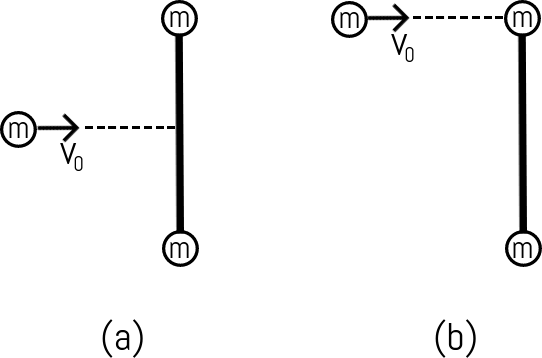
\includegraphics[scale=0.4]{fig1}
 \caption{(a) La colisión es a lo largo de la horizontal y justo en el punto medio 
 de la mancuerna. (b) La colisión es a lo largo de la horizontal y con la partícula 
 superior de la mancuerna. En ambos casos la mancuerna está inicialmente en reposo 
 respecto al sistema de laboratorio y está colocada perpendicularmente a la dirección 
 de impacto.}
\end{figure}

\vspace{.3cm}

\underline{Solución:} \vspace{.3cm}

En ambos casos tenemos un sistema cerrado en el cual se presenta una colisión 
elástica (no hay cambio en el estado interno de las partículas) sobre un piso sin
fricción, por lo tanto, al conocer estas condiciones del choque sabemos que la 
velocidad del centro de masa del sistema no cambia luego de la colisión, se 
debe conservar la energía cinética, el impulso lineal y ya que el sistema es 
cerrado también debe conservarse el impulso angular. 

\vspace{.3cm}

En este caso debido a la pregunta que nos hacen, es necesario calcular la 
velocidad del centro de masa de la mancuerna luego de la colisión. Desde un punto 
de vista cualitativo, el problema se puede resolver fácilmente al recordar los 
simples experimentos en colisiones. En el primer caso la partícula de masa 
$m$ choca en el medio de la mancuerna, que podemos considerar de masa $2m$, con 
lo cual intuitivamente sabemos que cuando un cuerpo de menor masa con una velocidad 
dada choca con un cuerpo de mayor masa en reposo, lo que ocurrirá, ya que el 
choque es elástico, es que la primera partícula rebotará y comenzará a moverse 
en sentido contrario, habiéndole transferido parte de su impulso lineal a la 
mancuerna, y debido a que se debe conservar el impulso y la energía cinética, 
es fácil ver que para contrarrestar el movimiento invertido de la primera partícula, 
la mancuerna debe moverse más rápido que la partícula, ya que el la velocidad del 
centro de masa no debe cambiar luego de la colisión. En el segundo caso, ya que 
el choque es en el extremo de la mancuerna, tenemos un choque elástico de 
partículas de igual masa donde una está en movimiento y la otra en reposo, y de 
nuevo recordando los experimentos clásicos sabemos que la primera partícula se 
detendrá y transferirá todo su impulso lineal a la partícula en reposo, pero debido 
al tipo de choque, la velocidad del centro de masa de la mancuerna, será menor 
que en el primer caso, ya que esto puede no ser tan intuitivo, hagamos unos pequeños 
cálculos.

\vspace{.3cm}

En el caso en que la partícula choca a la mancuerna en el centro, y debido a que 
la masa de la barra es despreciable, tenemos el choque de una partícula de masa $m$ con una 
de masa $2m$. Recordando las ecuaciones para la conservación del impulso lineal y que 
también por definición en un choque elástico la velocidad relativa de los dos cuerpos 
es igual y de signo contrario a la existente antes de él, 

\begin{equation}
 mv_{i1} + 2mv_{i2} = mv_{f1} + 2mv_{f_2},
\end{equation}

\begin{equation}
 v_{f1} - v_{f2} = - (v_{i1} - v_{i2}),
\end{equation}

que resultan en, 

\begin{equation}
 v_{1f} = \frac{(m - 2m)v_{1i} + 4mv_{i2}}{3m},
\end{equation}

\begin{equation}
  v_{2f} = \frac{(2m - m)v_{2i} + 2mv_{i1}}{3m},
\end{equation}

y al usar el hecho de que $v_{i2}$ es cero, 

\begin{equation}
 v_{1f} = - \frac{v_{1i}}{3} = - \frac{v_0}{3},
\end{equation}

\begin{equation}
  v_{2f} = \frac{2v_{i1}}{3} = \frac{2v_0}{3},
\end{equation}

tenemos que la velocidad del centro de masa de la mancuerna será, ya que pega justo en el 
medio de la misma, en el primer caso de $2/3$ de la velocidad inicial de la partícula.

\vspace{.3cm}

Ahora en el segundo caso, al chocar dos partículas de misma masa, tenemos 

\begin{equation}
 mv_{i1} + mv_{i2} = mv_{f1} + mv_{f_2},
\end{equation}

\begin{equation}
 v_{f1} - v_{f2} = - (v_{i1} - v_{i2}),
\end{equation}

que resultan en, 

\begin{equation}
 v_{1f} = \frac{\cancelto{0}{(m - m)}v_{1i} + 2mv_{i2}}{2m},
\end{equation}

\begin{equation}
  v_{2f} = \frac{\cancelto{0}{(m - m)}v_{2i} + 2mv_{i1}}{2m},
\end{equation}

y utilizando el hecho de que $v_{i2}$ es cero, 

\begin{equation}
 v_{1f} = 0,
\end{equation}

\begin{equation}
 v_{2f} = v_{1i} = v_0,
\end{equation}

que era lo que esperábamos. Entonces la velocidad de la mancuerna debe ser $v_0$ pero 
debido a que la masa de la mancuerna es de $2m$, la velocidad del centro de masa 
será $1/2v_0$.

\vspace{.3cm}

Por lo tanto ya que en el primer caso la velocidad del centro de masa de la mancuerna 
es de $2/3$ de la velocidad inicial, y en el segundo caso de $1/2$ de la velocidad 
inicial, en el primer caso la velocidad de centro de masa de la mancuerna será 
mayor.

\section{Problemas}

\subsection{Problema 1}

La interacción clásica entre dos átomos de un gas inerte, cada uno de masa $m$ está dada por el
potencial 

$$
V(r) = - \frac{2A}{r^6} + \frac{B}{r^{12}}
$$

con $A$ y $B$ constantes positivas y $r$ la separación entre los dos átomos, $r = |\overrightarrow{r_1} 
- \overrightarrow{r_2}|$.

\begin{enumerate}[label=\alph*)]
 \item Obtenga la hamiltoniana para el sistema de los dos átomos.
 \item Describa completamente el (los) estado(s) clásico(s) de energía mínima del presente 
 sistema.
 \item Si la energía es un poco mayor que la mínima, ¿Cuáles son las posibles frecuencias 
 del movimiento del sistema?
\end{enumerate}

\vspace{.3cm}

\underline{Solución:} \vspace{.3cm}

\begin{enumerate}[label=\alph*)]
 \item R:
\end{enumerate}

Podemos ver que tratamos con un sistema de fuerzas centrales de dos partículas ya que 
el potencial, y por ende la fuerza que existe entre los átomos de un gas inerte, está 
dirigida a lo largo de la línea que los conecta. Para describir un sistema de dos 
partículas generalmente necesitamos seis cantidades, en este caso escogeremos las 
tres componentes del de centro de masa del sistema $R$ y las tres componentes de 
la distancia relativa de las partículas $r = |\overrightarrow{r_1} - \overrightarrow{r_2}|$. 
Ahora debido a que el movimiento de traslación del sistema como un todo, no es muy 
interesante desde el punto de vista de la órbita de una partícula con respecto a la 
otra, escogeremos el origen del sistema de coordenadas en el centro de masa de 
las partículas, es decir que $R \equiv 0$. Y como es común en problemas de 
dos cuerpos donde solo actúan fuerzas centrales, podemos reducir el problema 
a uno equivalente de un cuerpo, en el cual solo debemos determinar el movimiento 
de una ``partícula'' de masa $\mu$ en el campo central descrito por la función 
potencial $V(r)$, donde $\mu$ es la masa reducida del sistema definida como 

\begin{equation}
 \mu \equiv \frac{m_1m_2}{m_1+m_2}.
\end{equation}

Por otra parte, debido a que la energía potencial solo depende de la distancia de 
la partícula al centro de fuerzas y no en la orientación, el sistema posee simetría 
esférica; esto es, que la rotación del sistema a lo largo de cualquier eje fijo 
a través del centro de fuerzas no puede afectar las ecuaciones de movimiento, y bajo 
estas condiciones el impulso angular del sistema se conserva. De esto, debe quedar 
claro que tanto el radio vector de la posición y el vector del impulso lineal 
de la partícula yace en un plano normal al impulso angular, que está fijo en el 
espacio, lo que significa que el movimiento en un campo central se da en un 
plano. En conclusión hemos reducido el problema a uno equivalente de una masa 
equivalente $\mu$ con dos grados de libertad, y por conveniencia podemos expresar 
la lagrangiana es coordenadas planas polares de la forma 

\begin{equation}
 L = \frac{1}{2}\mu(\dot{r}^2 + r^2\dot{\theta}^2) - V(r),
\end{equation}

y sustituyendo el potencial dado, tenemos que la lagrangiana del sistema será

\begin{equation}
 L = \frac{1}{2}\mu(\dot{r}^2 + r^2\dot{\theta}^2) + \frac{2A}{r^6} 
 - \frac{B}{r^{12}}.
\end{equation}

Para encontrar la hamiltoniana usamos la definición de impulso 

\begin{equation}
 p_i = \frac{\partial L}{\partial \dot{q}^i},
\end{equation}

para con esta cantidad, poder expresar las velocidades en término de los impulsos, y luego 
sustituir sus valores en la lagrangiana para obtenerla en términos de las posiciones 
e impulsos. Construimos así la hamiltoniana con la ecuación 

\begin{equation}
 H = \sum_i p_i\dot{q}^i(q,p,t) - L(q,p,t).
\end{equation}

Entonces tenemos, 

\begin{equation}
 p_r = \frac{\partial L}{\partial \dot{r}} = \mu\dot{r},
\end{equation}

de donde 

\begin{equation}
 \dot{r} = \frac{p_r}{\mu},
\end{equation}

y 

\begin{equation}
 p_\theta = \frac{\partial L}{\partial \dot{\theta}} = r^2\mu\dot{\theta},
\end{equation}

de donde 

\begin{equation}
 \dot{\theta} = \frac{p_\theta}{\mu r^2}.
\end{equation}

La hamiltoniana será entonces 

\begin{equation}
 H = p_r\dot{r} + p_\theta \dot{\theta} - L = 
 p_r\frac{p_r}{\mu} + p_\theta\frac{p_\theta}{\mu r^2} - 
 \frac{p_r^2}{2\mu} - \frac{p_\theta^2}{2\mu r^2} - \frac{2A}{r^6} 
 + \frac{B}{r^{12}}
\end{equation}

\begin{equation}
 \boxed{H = \frac{p_r^2}{2\mu} + \frac{p_\theta^2}{2\mu r^2} 
 -\frac{2A}{r^6}  + \frac{B}{r^{12}}.}
\end{equation}

\begin{enumerate}[label=\alph*)]
\setcounter{enumi}{1}
 \item R:
\end{enumerate}

El estado de energía mínima corresponde a $p_r = p_\theta = 0$, es decir que 
$T=0$, y ocurre en un $r_0$ que minimiza al potencial. Para obtener este $r_0$, 
resolvemos para $r_0$ la siguiente ecuación, 

\begin{equation}
 \frac{d}{dt}\left(-\frac{2A}{r^6} + \frac{B}{r^{12}} \right) = 0,
\end{equation}

\begin{equation}
 \frac{\cancel{12}A}{r^7} - \frac{\cancel{12}B}{r^{13}} = 0,
\end{equation}

de donde 

\begin{equation}
 A = \frac{B}{r_0^6},
\end{equation}

\begin{equation}
 \therefore r_0 = \left( \frac{B}{A}\right)^{1/6},
\end{equation}

entonces debido a que la lagrangiana no depende del tiempo y la energía cinética 
es una función cuadrática de las velocidades, la hamiltoniana será igual a la energía 
total del sistema, y el estado de energía mínima lo obtenemos sustituyendo el $r_0$ 
que obtuvimos (que representa la distancia entre los dos átomos para el estado de 
energía mínima clásica del sistema) en la hamiltoniana, que resulta en 

\begin{equation}
 H = \frac{-2A}{B/A} + \frac{B}{(B/A)^2},
\end{equation}

\begin{equation}
 \boxed{H = - \frac{A^2}{B}.}
\end{equation}

\begin{enumerate}[label=\alph*)]
\setcounter{enumi}{1}
 \item R:
\end{enumerate}

Si la energía es solo un poco mayor a la mínima, el sistema entrará en un régimen de 
oscilaciones pequeñas, donde la frecuencia normal del sistema será la de un oscilador 
armónico, 

\begin{equation}
 \omega = \sqrt{\frac{k}{\mu}},
\end{equation}

ahora sabemos que a primer orden 

\begin{equation}
 k = \left\zerodel\left(\frac{d^2V}{dr^2} \right)\right|_{r=r_0},
\end{equation}

entonces 

\begin{equation}
 k =  \left\zerodel\frac{d}{dr}\left(\frac{12A}{r^7} - \frac{12B}{r^{13}}\right)\right|_{r=r_0}
 = \frac{12}{r^7}\left\zerodel\frac{d}{dr}\left(A - \frac{B}{r^{6}}\right)\right|_{r=r_0}
\end{equation}

\begin{equation}
 k = \frac{12}{r^7}\left\zerodel\left(\frac{6B}{r^{7}}\right)\right|_{r=r_0}  
 = \left\zerodel\left(\frac{72B}{r^{14}}\right)\right|_{r=r_0}
\end{equation}

evaluando en $r_0$, 

\begin{equation}
 k = \frac{72B}{(B/A)^{7/3}} = \frac{72\cancel{B}}{(B/A)^{4/3}(\cancel{B}/A)},
\end{equation}

\begin{equation}
 \therefore k = 72A\left(\frac{A}{B}\right)^{4/3},
\end{equation}

y entonces la frecuencia del sistema si la energía es un poco mayor a la mínima 
será

\begin{equation}
 \boxed{\omega = \sqrt{\frac{72A}{\mu}\left(\frac{A}{B}\right)^{4/3}}.}
\end{equation}

\subsection{Problema 2}

Considere el siguiente sistema 

$$
L = \frac{m}{2}\dot{q}^2 - af(t)q
$$

con $f(t)$ una función arbitraria del tiempo pero integrable.

\begin{enumerate}[label=\alph*)]
 \item Considerando que una simetría del sistema es aquella que deja invariantes las 
 ecuaciones de movimiento. ¿Existe alguna simetría asociada a este sistema? Si es así,
 calcule la cantidad conservada correspondiente usando el teorema de Noether.
 \item Muestre que, efectivamente su derivada total con respecto del tiempo es cero.
 \item Construya el Hamiltoniano del sistema y escriba la ecuación de Hamilton-Jacobi 
 correspondiente.
 \item Resuelva la ecuación de hamilton-Jacobi y encuentre la funcional generadora de 
 tipo 2.
 \item Considere que $f(t) = \exp{(-bt)}$ con $b > 0$ y las condiciones iniciales
 $q(0) = \beta$ y $\dot{q}(0) = \rho$. Usando la teoría de Hamilton-Jacobi, encuentre 
 la trayectoria de la partícula.
\end{enumerate}

\vspace{.3cm}

\underline{Solución:} \vspace{.3cm}

\begin{enumerate}[label=\alph*)]
 \item R:
\end{enumerate}

Comencemos por obtener las ecuaciones de movimiento con la lagrangiana dada para 
tener un punto de comparación. Usando las ecuaciones de Lagrange 

\begin{equation}
 \frac{d}{dt}\left(\frac{\partial L}{\partial \dot{q}}\right) 
 - \frac{\partial L}{\partial q} = 0,
\end{equation}

\begin{equation}
 m\ddot{q} + af(t) = 0.
\end{equation}

Debido a que la lagrangiana depende explícitamente del tiempo, no existirán integrales 
de movimiento, sino sólo constantes de movimiento. Comúnmente las simetrías asociadas 
a constantes de movimiento son un poco menos obvias de encontrar, y en general éstas 
no provienen de una simetría en la forma estándar. En este caso podemos ver que 
la siguiente transformación, 

\begin{equation}
 Q = q + s,
\end{equation}

deja invariante a las ecuaciones de movimiento. Para ver esto, sustituyamos esta 
transformación en la lagrangiana original\footnote{$\frac{d}{dt}(Q -s) = \dot{Q}$},

\begin{equation}
 L' = \frac{m}{2}\dot{Q}^2 - af(t)(Q-s),
\end{equation}

y obtengamos las ecuaciones de movimiento desde las ecuaciones de Lagrange

\begin{equation}
 \frac{d}{dt}\left(\frac{\partial L'}{\partial \dot{Q}}\right) 
 - \frac{\partial L'}{\partial Q} = 0,
\end{equation}

que nos dan

\begin{equation}
 m\ddot{Q} + af(t) = 0.
\end{equation}

por lo tanto hemos demostrado que la transformación propuesta deja invariante a las 
ecuaciones de movimiento, y con la definición dada en el enunciado, vemos que es 
una simetría. Debido a que tratamos con una constante y no una integral de movimiento, 
la ecuación para obtener la cantidad conservada con el teorema de Noether será 

\begin{equation}
 I = \left(\left\zerodel\frac{\partial L'}{\partial \dot{Q}}
 \frac{\partial Q}{\partial s}\right)\right|_{s=0} - G,
\end{equation}

donde en este caso es fácil ver que $\frac{dG}{dt} = - af(t)$, ya que al sustituir 
y hacer los cálculos de las derivadas, tenemos que 

\begin{equation}
 \boxed{I = m\dot{Q} + a\int f(t) dt,}
\end{equation}

y entonces 

\begin{enumerate}[label=\alph*)]
\setcounter{enumi}{1}
 \item R:
\end{enumerate}

\begin{equation}
 \frac{dI}{dt} = m\ddot{Q} + af(t) = 0,
\end{equation}

que es cero debido a la ecuación de movimiento obtenida.

\begin{enumerate}[label=\alph*)]
\setcounter{enumi}{2}
 \item R:
\end{enumerate}

Para encontrar la hamiltoniana usamos la definición de impulso 

\begin{equation}
 p = \frac{\partial L}{\partial \dot{q}},
\end{equation}

para con esta cantidad, poder expresar la velocidad en término del impulso, y luego 
sustituir su valor en la lagrangiana para obtenerla en términos de las posiciones 
e impulsos, construimos así la hamiltoniana con la ecuación 

\begin{equation}
 H = p\dot{q}(q,p,t) - L(q,p,t).
\end{equation}

Tenemos entonces que 

\begin{equation}
 p = \frac{\partial L}{\partial \dot{q}} = m\dot{q},
\end{equation}

y 

\begin{equation}
 \dot{q} = \frac{p}{m},
\end{equation}

\begin{equation}
 \therefore L = \frac{p^2}{2m} - af(t)q,
\end{equation}

y

\begin{equation}
 H = p\frac{p}{m} - \frac{p^2}{2m} + af(t)q,
\end{equation}

\begin{equation}
 \boxed{\therefore H = \frac{p^2}{2m} + af(t)q.}
\end{equation}

Para construir la ecuación de Hamilton-Jacobi, transformamos los impulsos por 
$\frac{\partial S}{\partial q}$ y hacemos uso de la ecuación 

\begin{equation}
 H\left(q,\frac{\partial S}{\partial q},t\right) = - \frac{\partial S}{\partial t},
\end{equation}

donde $S$ es una función generadora de transformaciones canónicas y una solución 
completa de la ecuación. Entonces 

\begin{equation}
 \boxed{\frac{1}{2m}\left(\frac{\partial S}{\partial q}\right)^2 + af(t)q = 
 - \frac{\partial S}{\partial t}.}
\end{equation}

\begin{enumerate}[label=\alph*)]
\setcounter{enumi}{3}
 \item R:
\end{enumerate}

Debido a que la ecuación de Hamilton-Jacobi es dependiente del tiempo, proponemos 
una solución del tipo 

\begin{equation}
 S(q,t) = A(t)q + B(t),
\end{equation}

entonces la ecuación de Hamilton-Jacobi se transforma en

\begin{equation}
\frac{1}{2m} A^2 + af(t)q + \dot{A}q + \dot{B} = 0,
\end{equation}

\begin{equation}
 \therefore [af(t) + \dot{A}]q + \left[\frac{1}{2m}A^2 + \dot{B} \right] = 0,
\end{equation}

y para que esta ecuación los coeficientes de $q$ y de $1$ deben ser idénticamente 
cero, por lo tanto\footnote{Llamaremos $\int f(t) dt = F(t)$.}

\begin{equation}
 \dot{A} + af(t) = 0 \Rightarrow dA = - a\int f(t)dt
\end{equation}

\begin{equation}
 \therefore A = -aF(t) + A_0.
\end{equation}

Y por otra parte, utilizando que $A^2 = a^2F^2 - 2aFA_0 + A_0^2$, 

\begin{equation}
 \dot{B} + \frac{1}{2m}A^2 = 0 \Rightarrow dB = 
 - \frac{1}{2m} \int [a^2F^2 - 2aFA_0 + A_0^2] dt
\end{equation}

Y entonces 

\begin{equation}
 \boxed{S = [-aF(t) + A_0]q  - \frac{1}{2m} \int [a^2F^2 - 2aFA_0] dt - \frac{1}{2m}A_0^2t.}
\end{equation}

Como es de costumbre en la formulación de Hamilton-Jacobi, calculamos el impulso 
con 

\begin{equation}
 \boxed{p = \frac{\partial S}{\partial q} = -aF(t) + A_0,}
\end{equation}

y terminamos de calcular la trayectoria con 

\begin{equation}
 \xi = \frac{\partial S}{\partial A_0} = q + \frac{a}{m}\int F dt - \frac{A_0t}{m},
\end{equation}

por lo tanto 

\begin{equation}
 \boxed{q = \xi - \frac{a}{m}\int F dt + \frac{A_0t}{m}.}
\end{equation}

\begin{enumerate}[label=\alph*)]
\setcounter{enumi}{4}
 \item R:
\end{enumerate}

Si $f(t) = \exp{(-bt)}$, tenemos que $F(t) = - \frac{1}{b}\exp{(-bt)}$, y 

\begin{equation}
 \boxed{p = a\frac{1}{b}\exp{(-bt)} + A_0,}
\end{equation}

\begin{equation}
 \boxed{q = \xi - \frac{a}{mb^2}\exp{(-bt)} + \frac{A_0t}{m}.}
\end{equation}

Para aplicar las condiciones iniciales calculamos primero

\begin{equation}
 \dot{q} = \frac{a}{mb}\exp{(-bt)} + \frac{A_0}{m},
\end{equation}

Aplicando la primera condición inicial $q(0) = \beta$, tenemos que 

\begin{equation}
 \xi - \frac{a}{mb^2} = \beta \Rightarrow \xi = \beta + \frac{a}{mb^2},
\end{equation}

y aplicando la segunda $\dot{q}(0) = \rho$, 

\begin{equation}
\frac{a}{mb} + \frac{A_0}{m} = \rho \Rightarrow A_0 = m\rho - \frac{a}{b}, 
\end{equation}

entonces 

\begin{equation}
 \boxed{q(t) = \beta + \frac{a}{mb^2} - \frac{a}{mb^2}\exp{(-bt)} + 
 \left(\rho - \frac{a}{mb} \right)t.}
\end{equation}

\subsection{Problema 3}

Una partícula de masa $m$ está restringida a moverse en el interior de un riel circular 
de radio $R$. El riel circular está fijado al piso en posición vertical. Un pequeño 
motor hacer girar el riel en torno al eje de simetría vertical con rapidez angular 
constante $\omega$ (ver figura). Considere el cero de energía potencial en el piso y 
sea $\theta$ el ángulo que forma el radio vector de posición de la partícula con el 
eje de rotación.

\begin{figure}[H]
 \center 
 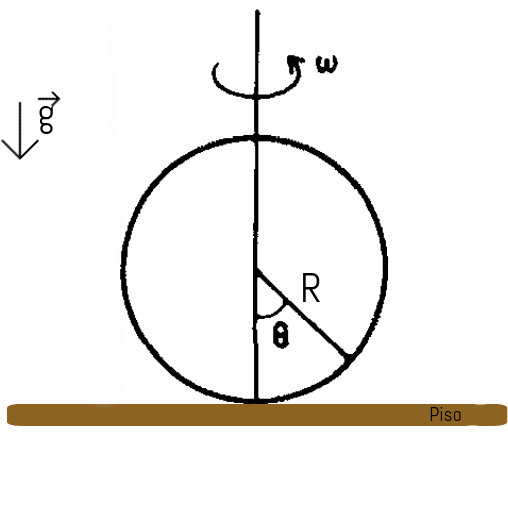
\includegraphics[scale=0.5]{fig2}
 \caption{El riel circular gira en torno al eje de simetría vertical con rapidez 
 angular constante $\omega$. El punto de contacto entre el riel y el piso es 
 fijo (i.e., no se desplaza).}
\end{figure}

\begin{enumerate}[label=\alph*)]
 \item Determine el Lagrangiano del sistema con constricción y la ecuación de movimiento 
 en $\theta$ para la partícula.
 \item Para que exista una órbita a $\theta_{eq}= \text{cte}$ y distinta de cero, $\omega$
 tiene que ser mayor que cierta $\omega_0$. Determine $\omega_0$.
\end{enumerate}

\vspace{.3cm}

\underline{Solución:} \vspace{.3cm}

\begin{enumerate}[label=\alph*)]
 \item R:
\end{enumerate}

Debido a que la única fuerza que existe es la gravitacional, el potencial se 
escribiría como (utilizando coordenadas esféricas)

\begin{equation}
 V = mgz = mgR\cos{\theta},
\end{equation}

ahora debido a que se solicita que el cero de la energía potencial esté en el piso, 
hay que cambiar el punto de referencia para el potencial, y ya que al potencial 
gravitacional solo le importa la diferencia entre el punto de referencia y el suelo, 
para acomodar esta condición hacemos primero,

\begin{equation}
 V = mg(z - z_0),
\end{equation}

donde el $z_0$ en este caso será $-R$ ya que el eje $z$ se ha tomando como positivo 
hacia arriba, entonces 

\begin{equation}
 V = mg(z + R) = mg(R\cos{\theta} + R),
\end{equation}

\begin{equation}
 \therefore V = mgR(\cos{\theta} + 1).
\end{equation}

La energía cinética del sistema se escribe como 

\begin{equation}
 T = \frac{m}{2}(\dot{x}^2 + \dot{y}^2 + \dot{z}^2),
\end{equation}

debido a que existe la constricción de que $R = \text{cte}$, y recordamos que 
estamos usando coordenadas esféricas, tenemos que 

\begin{align*}
 \dot{x} &= R\dot{\theta}\cos{\theta}\cos{\phi} - R\dot{\phi}\sen{\theta}\sen{\phi}, \\
 \dot{y} &= R\dot{\theta}\cos{\theta}\sen{\phi} + R\dot{\phi}\sen{\theta}\cos{\phi}, \\
 \dot{z} &= - R\dot{\theta}\sen{\theta}.
\end{align*}

Entonces la energía cinética se transforma en (usando el hecho de que la velocidad 
angular es constante y por lo tanto $\dot{\phi} = \omega$),

\begin{equation}
 T = \frac{1}{2}m\left[R\dot{\theta} + R^2\omega^2\sen^2{\theta} \right],
\end{equation}

por lo que la lagrangiana del sistema será

\begin{equation}
 L = T - V = \frac{1}{2}m\left[R\dot{\theta} + R^2\omega^2\sen^2{\theta} \right] 
 -  mgR(\cos{\theta} + 1).
\end{equation}

Y las ecuaciones de movimiento las obtenemos con la ecuación de Lagrange para 
$\theta$, 

\begin{equation}
 \frac{d}{dt}\left(\frac{\partial L}{\partial \dot{\theta}}\right) - 
 \frac{\partial L}{\partial \theta} = 0,
\end{equation}

\begin{equation}
 \frac{d}{dt}\left( m\dot{\theta}R^2 \right) - 
 - mR^2\omega^2\sen{\theta}\cos{\theta} + mgR\sen{\theta}  = 0,
\end{equation}

\begin{equation}
 \boxed{\therefore R\ddot{\theta} - R\omega^2\sen{\theta}\cos{\theta} + g\sen{\theta}
 = 0.}
\end{equation}

\begin{enumerate}[label=\alph*)]
\setcounter{enumi}{1}
 \item R:
\end{enumerate}

La energía total del sistema es 

\begin{equation}
 E = T + V =  \frac{1}{2}m\left[R\dot{\theta} + R^2\omega^2\sen^2{\theta} \right] 
 +  mgR(\cos{\theta} + 1),
\end{equation}

de donde vemos que podemos estudiar este sistema como uno con potencial efectivo 

\begin{equation}
 V_{ef} =  \frac{1}{2}mR^2\omega^2\sen^2{\theta}  +  mgR(\cos{\theta} + 1),
\end{equation}

para calcular $\omega_0$, debemos derivar $V_{ef}$ con respecto a $\theta$ e 
igualar a cero, con lo cual obtendremos el ángulo de equilibrio y con esto 
podemos saber en que rangos se encontrará la frecuencia solicitada.

\begin{equation}
 \frac{d}{d\theta} \left[\frac{1}{2}mR^2\omega^2\sen^2{\theta} + 
 mgR(\cos{\theta} + 1) \right] = 0,
\end{equation}

\begin{equation}
 \cancel{m}R^{\cancel{2}}\omega^2\cancel{\sen{\theta}}\cos{\theta} - \cancel{m}\cancel{R} 
 g\cancel{\sen{\theta}} = 0,
\end{equation}

\begin{equation}
 R\omega^2\cos{\theta} - g = 0,
\end{equation}

de donde vemos que 

\begin{equation}
 \theta = \arccos{\left[\frac{g}{R\omega^2}\right]},
\end{equation}

con lo cual, debido a la definición de $\arccos$ que 

\begin{equation}
 \frac{g}{R\omega^2} < 1,
\end{equation}

y entonces 

\begin{equation}
 \boxed{\omega_0 > \sqrt{\frac{g}{R}}.}
\end{equation}

\end{document}